
%(BEGIN_QUESTION)
% Copyright 2009, Tony R. Kuphaldt, released under the Creative Commons Attribution License (v 1.0)
% This means you may do almost anything with this work of mine, so long as you give me proper credit

In relay ladder logic (RLL) programming, it is considered bad practice to have multiple instances of an identical (standard) ``relay'' coil in a program:

$$\includegraphics[width=15.5cm]{i02376x01.eps}$$

Explain why this is considered poor practice in PLC programming.  Next, determine the status of the {\tt Pump\_run} output channel given the following bit states:

\begin{itemize}
\item{} {\tt Timer\_01} = {\tt 1}
\item{} {\tt Level\_low} = {\tt 1}
\item{} {\tt Switch\_hand} = {\tt 0}
\item{} {\tt OL\_contact} = {\tt 0}
\item{} {\tt Sump\_wet} = {\tt 0} 
\end{itemize}

\vfil

\underbar{file i02376}
\eject
%(END_QUESTION)





%(BEGIN_ANSWER)

This is a graded question -- no answers or hints given!

%(END_ANSWER)





%(BEGIN_NOTES)

Multiple instances of a coil in RLL programming means the possibility exists for different Boolean values to be written to the same bit in memory.  In other words, one rung of logic might be telling the pump to run, while another might be telling it to not run.  This makes the {\tt Pump\_run} bit liable to change within one scan of the program, with only the last scanned (evaluated) value being the one sent to the PLC discrete output channel.

\vskip 10pt

In this particular example, the {\tt Pump\_run} bit will be in the set state ({\tt 1}) at the conclusion of the program scan because the {\it last} rung in this program is ``energizing'' the {\tt Pump\_run} coil.  The coil in the first run is ``de-energized,'' making the {\tt Pump\_run} bit a {\tt 0} state during the rest of the program, but that is of no consequence to the output state because the output register gets updated only after the entire program has been scanned.

%INDEX% PLC, ladder logic programming: avoiding multiple coils of the same label in a program

%(END_NOTES)


